\documentclass[11pt]{article}

\usepackage[utf8x]{inputenc}
\usepackage{graphicx}
\usepackage{url}
\usepackage{amsmath}

\title{VisibleSim Manual}
\author{Julien Bourgeois, Benoît Piranda, Thadeu Knychala Tucci, André Naz}

\begin{document}

\maketitle

\newpage
\tableofcontents
\newpage

\section{Introduction}

VisibleSim is a general discrete event simulator (DES) for modular robot systems.

\section{Installation}

\section{User applications in VisibleSim}

\subsection{Examples of applications}

\subsection{Implementing a new application}

\subsection{Running an application}
\subsubsection{C++ application}
\subsubsection{Meld application}
\subsubsection{Command line arguments}

\section{Embedded debugger}

\section{Local clock Simulation}

VisibleSim supports local clock simulation. This section details the clock model used by the simulator. The programming API is available in VisibleSim Doxygen documentation.

\subsection{Systematic model for clocks}

\cite{allan1987time} proposes a general model for oscillators:
\begin{equation}
x(t) = x_0 + y_0t + \frac{1}{2}Dt^2 + \epsilon(t)
\label{eq:oscillator-model}
\end{equation}
where $t$ is the simulation time (real-time), $x(t)$ is the local time, $x_0$ is the time offset, $y_0$ is the frequency offset, $D$ is the frequency drift and $\epsilon(t)$ is the random noise. $\epsilon(t)$ is a not deterministic. \cite{ring2010clock} suggests to measure the Power Spectral Density (PSD) of the noise $S_y(f)$ and to design a filter with the frequency response $H(f)$ to simulate the oscillator noise.

%not true: \cite{ma2007understanding} assume that $\epsilon(t)$ follows a Gaussian distribution $\mathcal{N}(0,\sigma^2)$.

\subsection{Model parameter estimation through experiments}

We used hardware Blinky Blocks to compute realistic clock models. Blinky Blocks are equipped with a micro-controller ATxmega256A3 that holds a 16-bit Real Time Counter (RTC). The RTC can be plugged to different oscillators. We choose to study clock behavior using the most precise internal oscillator available: a 32.768 kHz (actually divided down to 1.024 kHz) calibrated RC oscillator with a precision of 1\%  (at 3V and 25°C) and a resolution of 1 ms\footnote{see AVR1003: Using the XMEGA$^{TM}$ Clock System (\url{http://www.atmel.com/images/doc8072.pdf}) for more details.}.

Typical RC oscillators are cheap, but generally suffer from poor accuracy over temperature and supply voltage. Moreover, they generally show important variations of nominal output frequency\footnote{see \url{http://www.maximintegrated.com/en/app-notes/index.mvp/id/2154} for more details.}.

We conducted experiments on hardware Blinky Blocks in order to compute model parameters. We used a system composed of 6 blocks to collect time reference points $<t,x^i(t)>$ with $i$ the block unique identifier every 5 seconds during 24 hours. The real-time $t$ was provided by a computer. We assume the computer clock to be perfect. The set of blocks were powered with 5V and 0.36A. We observed that the behavior of the clock of a block varies slightly from an execution to another. The variations seems independent from the location of the block in the system, from the distance to the block plugged to the power supply, and from the distance to the block that receives the real-time $t$. Figure \ref{fig:drift-noise} shows the clock drift and the noise $\epsilon(t)$ distribution.  We assume that Blinky Blocks clocks follow \eqref{eq:oscillator-model}'s model. We decided to model noise using a normal law $\mathcal{N}(0,(residual\ standard\ error)^2)$. Figure \ref{fig:parameter-values} shows experimental parameter values using polynomial regression. 

\begin{figure}[h!]
\centering
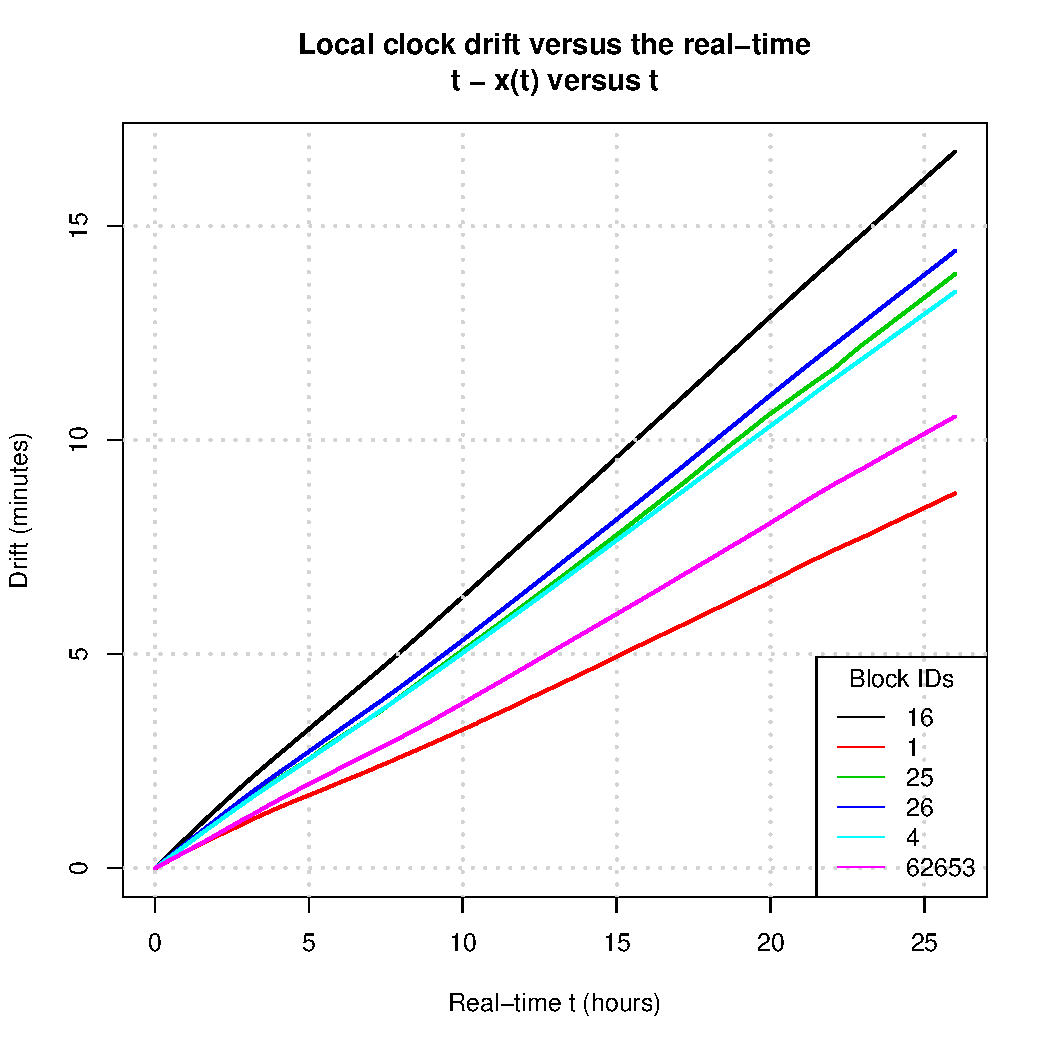
\includegraphics[width=0.49\textwidth]{pictures/drift.pdf}
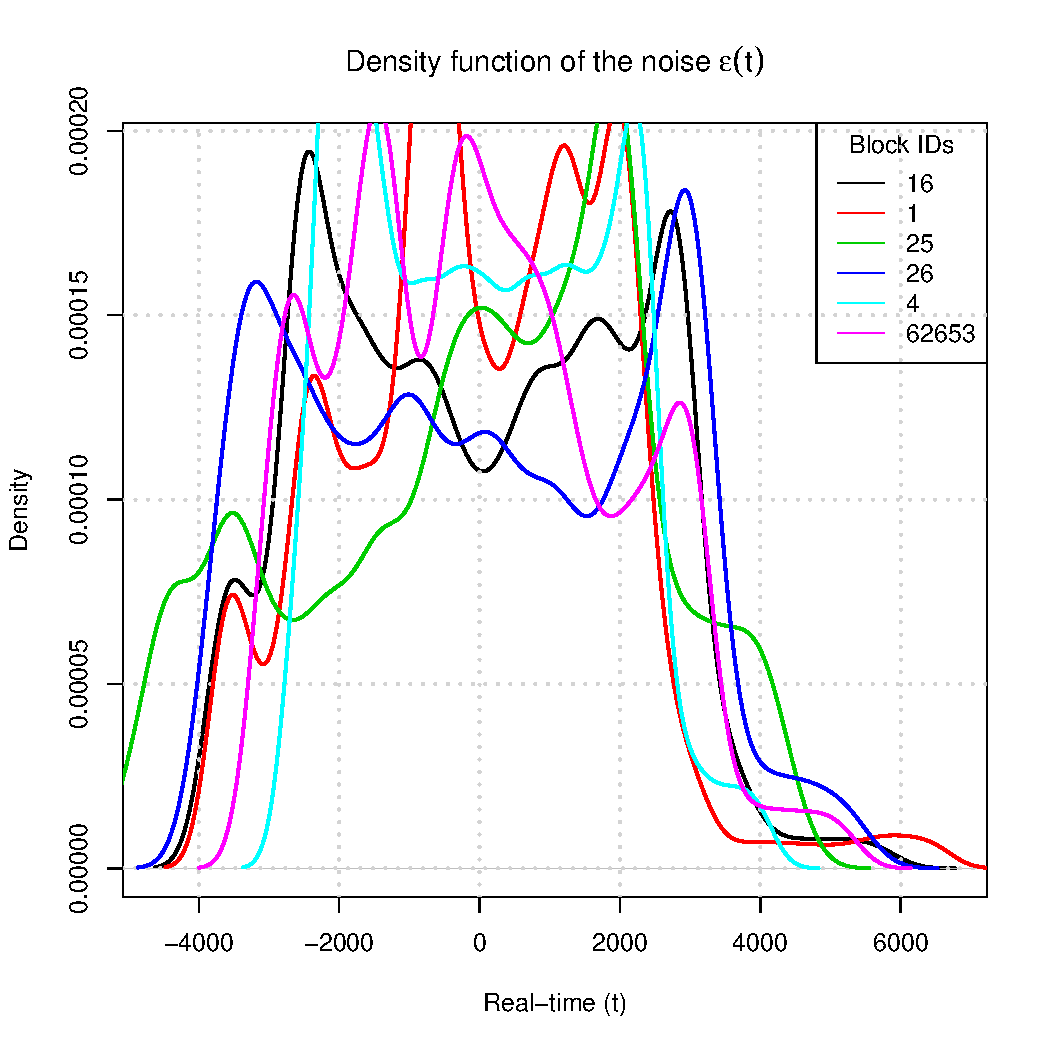
\includegraphics[width=0.49\textwidth]{pictures/noise.pdf}
\caption{Local clock drift (t - x(t)) and noise ($\epsilon(t)$) distribution.}
\label{fig:drift-noise}
\end{figure}

\begin{figure}[h!]
\scriptsize
\begin{center}
\begin{tabular}{|c|c|c|c|c|} 
\hline
Parameter & Min & Mean & Max & Standard-deviation \\
\hline
$D\ (ms^{-1})$ & -1.613992e-11 & -1.179717e-11 & -7.991859e-12 & 3.060884e-12 \\
\hline
$y_0\ (none)$ & 0.9896537 & 0.9922277 & 0.9949096 & 0.001851285\\
\hline
$x_0\ (ms)$ & -5984.141 & -3532.051 & -785.9812 & 1921.629\\
\hline
Residual standard error $(ms)$ & 1688.103 &  2080.197  & 2423.646 & 294.832\\
\hline
\end{tabular}
\end{center}
\label{fig:parameter-values}
\caption{Parameters}
\end{figure}

Figure \ref{fig:parameter-distribution} shows the distribution of the parameter values. The parameters $D$, $y_0$ and the residual standard error seems normally distributed. As a consequence, we randomly generate clock parameters according to normal laws with the corresponding mean and standard deviation.

\begin{figure}[h!]
\centering
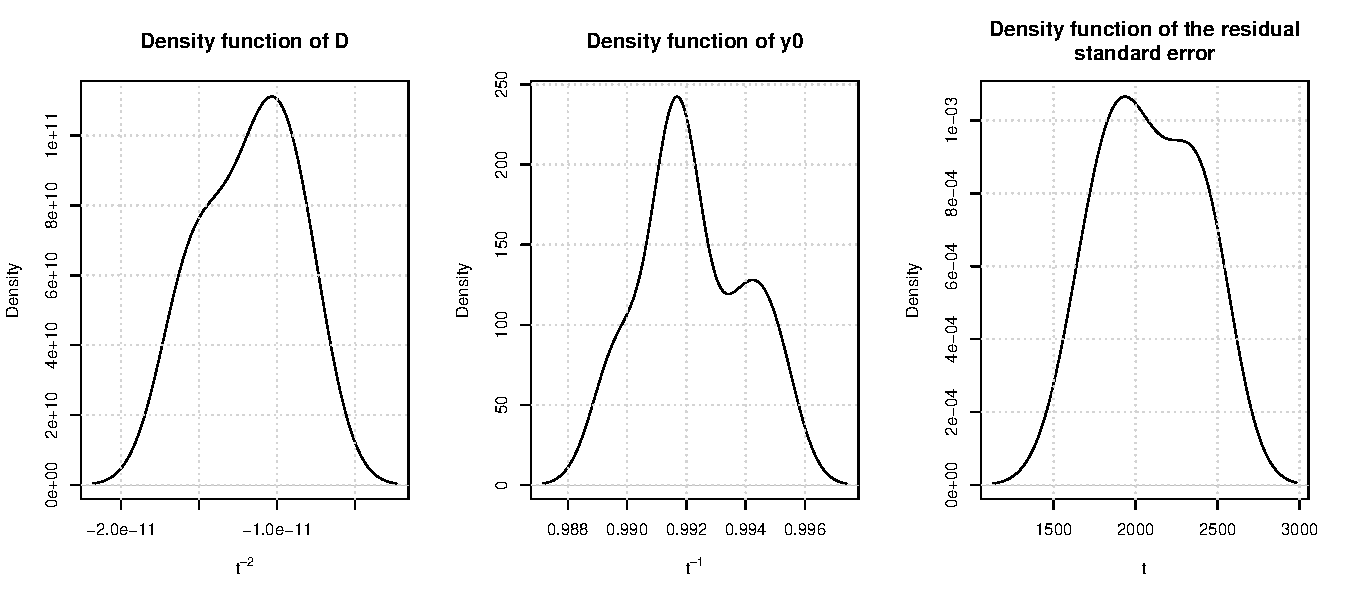
\includegraphics[width=\textwidth]{pictures/parameters.pdf}
\caption{Parameter distributions.}
\label{fig:parameter-distribution}
\end{figure}

\newpage

\subsection{Clock simulation in DES}

\cite{ring2010clock} explains how to enhance DES with efficient local clock simulation. For a given simulation and a given block $i$, Points in time need to be consistent:

\begin{equation}
t_2 < t_1 \iff x^i(t_2) \leq x^i(t_1)
\label{eq:consistency-lessthan}
\end{equation}

\begin{equation}
t_2 = t_1 \iff x^i(t_2) = x^i(t_1)
\label{eq:consistency-equalto}
\end{equation}

\begin{equation}
t_2 > t_1 \iff x^i(t_2) \geq x^i(t_1)
\label{eq:consistency-greaterthan}
\end{equation}

Consistency equations \eqref{eq:consistency-lessthan} \eqref{eq:consistency-equalto} \eqref{eq:consistency-greaterthan} are obvious but not trivial to ensure when considering noise simulation. For example, if we consider that $t_2 = t_1 + 1$, $D > 0$, $y_0 > 0$, $\epsilon(t_1) > 0$ and $\epsilon(t_2) < 0$, then $x(t_2) < x(t_1)$ which is inconsistent.

\cite{ring2010clock} proposes to use a caching strategy by storing the last calculated simulation times and local times. These reference points are then used to ensure time consistency. We use that approach in VisibleSim.

\bibliographystyle{plain}
\bibliography{manual}

\end{document}
